\definecolor{maincolor}{HTML}{A955FF}
\definecolor{maincolor2}{HTML}{FFA200}
\definecolor{maincolor3}{HTML}{EE005F}
\definecolor{maincolor4}{HTML}{8E3400}


\begin{figure*}[t]
\pgfplotsset{width=6.06cm,height=6cm,
    every axis y label/.append style={at={(-0.09,0.5)}},
    every axis/.append style={line width=0.6pt},%边框线段粗细
}
\centering
\subfigure[EnDe]{%设置子图以及子图标题
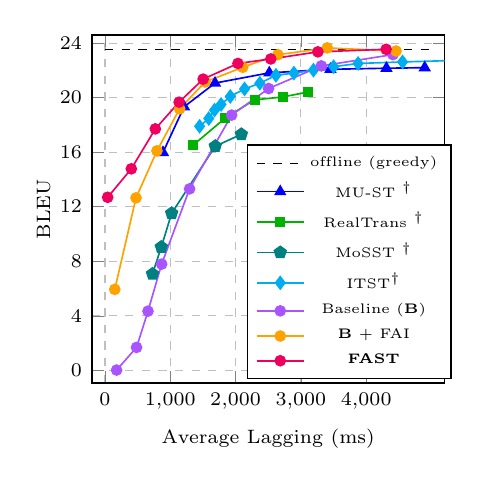
\begin{tikzpicture}[baseline]
\begin{axis}[
    ylabel=BLEU,%y轴标签名
    xlabel=Average Lagging (ms),
    enlargelimits=0.04,
    font=\scriptsize,
    legend style={font=\tiny,
    at={(0.73,0.01)},
    anchor=south,
    legend columns=1},
    xmajorgrids=true,%x轴网格线
    ymajorgrids=true,%y轴网格线
    grid style=dashed,%虚线
    xmin=0, xmax = 5000,
    xtick={0,1000,2000,3000,4000},
    ytick={0,4,8,12,16,20,24},%刻度值,在ymin和ymax之间随意设置,若未设置ymin和ymax则可能不会生效
]
\addplot[color=black,dashed,line width=0.6pt] coordinates {(1,23.53)(5000,23.53)};
\addplot[color=blue,mark=triangle*,line width=0.6pt] coordinates{(888,15.98)(1211,19.33)(1685,21.07)(2516,21.82)(3452,22.08)(4310,22.16)(4896,22.20)};%MU-ST
\addplot[color=green!70!black,mark=square*, mark size=1.5pt,line width=0.6pt] coordinates {(1355,16.54)(1838,18.49)(2290,19.84)(2720,20.05)(3106,20.41)};%RealTrans Wait-k-stride-3
\addplot[color=teal,mark=pentagon*, mark size=2.2pt,line width=0.6pt] coordinates {(728,7.07)(862,9.04)(1021,11.52)(1689,16.44)(2088,17.31)}; % official MoSST 
\addplot[color=cyan,mark=diamond*, mark size=2.2pt,line width=0.6pt] coordinates {(1449,17.9)(1589,18.47)(1678,19.09)(1778,19.5)(1919,20.09)(2137,20.64)(2371,21.06)(2618,21.64)(2893,21.8)(3193,22.02)(3501,22.27)(3876,22.51)(4557,22.62)(5206,22.71)}; % ITST
\addplot[color=maincolor,mark=*, mark size=1.8pt,line width=0.6pt] coordinates {(178,0.02)(483.4,1.68)(658.6,4.34)(867.43,7.79)(1295.16,13.31)(1939.46,18.72)(2505.04,20.67)(3312.15,22.33)(4409.65,23.16)}; % Our MoSST 
\addplot[color=maincolor2,mark=*, mark size=1.8pt,line width=0.6pt] coordinates {(150,5.94)(475,12.65)(795.84,16.1)(1143.37,19.19)(1533.63,21.15)(2109.41,22.23)(2647.03,23.15)(3403.9,23.65)(4457.14,23.42)}; %Baseline + FAI
\addplot[color=maincolor3,mark=*, mark size=1.8pt,line width=0.6pt] coordinates {(41,12.69)(403,14.78)(771,17.71)(1135,19.67)(1503,21.36)(2036,22.51)(2539,22.84)(3260,23.36)(4305,23.55)}; % FAST FAD+FAI

\legend{offline (greedy),MU-ST $^{\dagger}$,RealTrans $^{\dagger}$,MoSST $^{\dagger}$, ITST$^{\dagger}$,Baseline (\textbf{B}),\textbf{B} + FAI,\textbf{FAST}}
\end{axis}
\end{tikzpicture}}
~
\subfigure[EnEs]{%设置子图以及子图标题
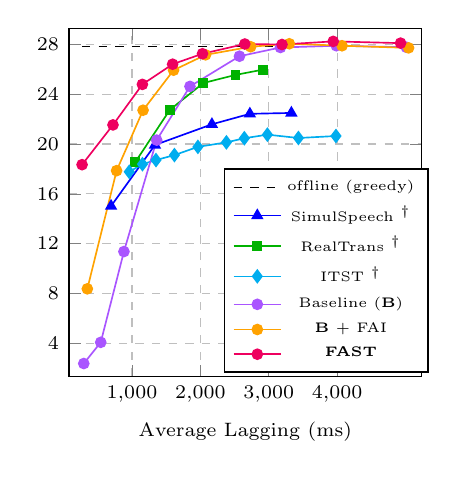
\begin{tikzpicture}[baseline]
\begin{axis}[
    % ylabel=BLEU,%y轴标签名
    xlabel=Average Lagging (ms),
    enlargelimits=0.04,
    font=\scriptsize,
    legend style={font=\tiny,
    at={(0.73,0.01)},
    anchor=south,
    legend columns=1},
    xmajorgrids=true,%x轴网格线
    ymajorgrids=true,%y轴网格线
    grid style=dashed,%虚线
    % xmin=700, xmax = 4500,
    xtick={0,1000,2000,3000,4000},
    ytick={0,4,8,12,16,20,24,28},%刻度值,在ymin和ymax之间随意设置,若未设置ymin和ymax则可能不会生效
]
\addplot[color=black,dashed,line width=0.6pt] coordinates {(270,27.81)(4000,27.81)};
\addplot[color=blue,mark=triangle*,line width=0.6pt] coordinates{(694,15.02)(1336,19.92)(2169,21.58)(2724,22.42)(3331,22.49)};%SimulSpeech
\addplot[color=green!70!black,mark=square*, mark size=1.5pt,line width=0.6pt] coordinates {(1047,18.54)(1554,22.74)(2043,24.89)(2514,25.54)(2920,25.97)};%RealTrans Wait-k-stride-2
\addplot[color=cyan,mark=diamond*, mark size=2.2pt,line width=0.6pt] coordinates {(960,17.77)(1153,18.38)(1351,18.71)(1621,19.11)(1964,19.77)(2381,20.13)(2643,20.46)(2980,20.75)(3434,20.48)(3983,20.64)}; % ITST
\addplot[color=maincolor,mark=*, mark size=1.8pt,line width=0.6pt] coordinates {(295,2.39)(543,4.09)(882,11.37)(1361,20.31)(1848,24.62)(2572,27.04)(3171,27.74)(3988,27.88)(5012,27.76)}; % Our MoSST
\addplot[color=maincolor2,mark=*, mark size=1.8pt,line width=0.6pt] coordinates {(347,8.38)(775,17.86)(1162,22.71)(1608,25.92)(2076,27.15)(2736,27.8)(3301,28.04)(4072,27.88)(5045,27.71)}; %Baseline + FAI
\addplot[color=maincolor3,mark=*, mark size=1.8pt,line width=0.6pt] coordinates {(270,18.34)(722,21.53)(1152,24.78)(1594,26.4)(2031,27.24)(2650,28.02)(3194,27.98)(3943,28.23)(4928,28.09)}; % FAST FAD+FAI

\legend{offline (greedy),SimulSpeech $^{\dagger}$,RealTrans $^{\dagger}$,ITST $^{\dagger}$,Baseline (\textbf{B}),\textbf{B} + FAI,\textbf{FAST}}
\end{axis}
\end{tikzpicture}}
~
\subfigure[EnFr]{%设置子图以及子图标题
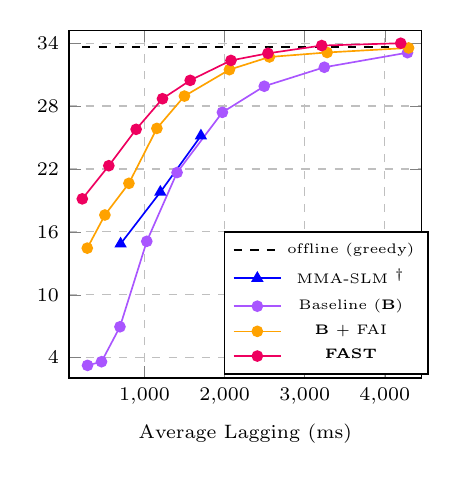
\begin{tikzpicture}[baseline]
\begin{axis}[
    % ylabel=BLEU,%y轴标签名
    xlabel=Average Lagging (ms),
    enlargelimits=0.04,
    font=\scriptsize,
    legend style={font=\tiny,
    at={(0.73,0.01)},
    anchor=south,
    legend columns=1},
    xmajorgrids=true,%x轴网格线
    ymajorgrids=true,%y轴网格线
    grid style=dashed,%虚线
    % xmin=700, xmax = 4500,
    % xtick={0,1000,2000,3000,4000,5000,6000},
    ytick={4,10,16,22,28,34},%刻度值,在ymin和ymax之间随意设置,若未设置ymin和ymax则可能不会生效
]
\addplot[color=black,dashed,line width=0.6pt] coordinates {(220,33.63)(4200,33.63)};
\addplot[color=blue,mark=triangle*,line width=0.6pt] coordinates{(701,14.86)(1197,19.79)(1704,25.16)};% MMA-SLM
\addplot[color=maincolor,mark=*, mark size=1.8pt,line width=0.6pt] coordinates {(288,3.27)(463,3.62)(693,6.95)(1028,15.1)(1406,21.66)(1972,27.4)(2495,29.89)(3245,31.7)(4283,33.09)}; % baseline=our mosst
\addplot[color=maincolor2,mark=*, mark size=1.8pt,line width=0.6pt] coordinates {(285,14.45)(505,17.61)(805,20.63)(1154,25.87)(1498,28.95)(2060,31.47)(2559,32.68)(3280,33.11)(4297,33.54)}; % + FAI
\addplot[color=maincolor3,mark=*, mark size=1.8pt,line width=0.6pt] coordinates {(223,19.15)(554,22.31)(895,25.78)(1224,28.7)(1570,30.45)(2079,32.35)(2541,33.03)(3212,33.77)(4199,33.99)}; % FAST 

\legend{offline (greedy),MMA-SLM $^{\dagger}$, Baseline (\textbf{B}),\textbf{B} + FAI,\textbf{FAST}}

\end{axis}
\end{tikzpicture}}
\caption{The translation quality (BLEU) against the latency metrics (AL) on the tst-COMMON set of MuST-C EnDe, EnEs, and EnFr dataset. 
$^{\dagger}$ denotes that the results are obtained from corresponding papers.
offline is the offline performance of teacher model (offline-trained ST) by greedy search. 
The curve corresponding to \textbf{B} is the online performance of the teacher model using vanilla \textit{wait-k} policy. 
The curve corresponding to \textbf{B} + FAI is the online performance of the teacher model with our FAI strategy.
The curve corresponding to \textbf{FAST} is the online performance of our student model with the FAI strategy, \emph{i.e.}, FAD + FAI.}
\label{fig:main_results}
\end{figure*}


